\chapter{Investigações preliminares em motivação em ensino STEM}

Este capítulo descreve as investigações preliminares que foram realizadas com intenção de verificar o ensino de STEM, em especial a motivação destes estudantes e a questão da igualdade de gênero nestas áreas. Na seção 2.1 é apresentado o estado atual da participação feminina nas áreas de STEM, algumas iniciativas que visam melhorar a lacuna existente e também é detalhado o projeto criado a partir da tese e em parceria entre a UFRJ e o IST, denominado igualdade STEM. Na seção 2.2, é apresentado uma revisão em torno das principais teorias motivacionais aplicadas na área da educação em estudantes de STEM, principalmente a Teoria da Autodeterminação e a Teoria de Metas. Na seção 2.3, é apresentado o resultado das pesquisas relativas a quizzes aplicados em autorregulação da aprendizagem, através de um mapeamento sistemático. Na seção 2.4, é apresentado o as principais caraterísticas de plataformas de ensino online, em especial as plataforma de MOOC. Na seção 2.5, são apresentados os principais conceitos sobre narrativas e sua aplicação nas áreas da educação. Por último, na Seção 2.6 são feitas as considerações finais do capítulo.


\section{O Projeto IgualdadeStem}

Nos últimos anos, a diferença de gênero diminuiu globalmente, mas ainda há um longo caminho a percorrer até a paridade. No ritmo atual, levará 99,5 anos para fechar a lacuna globalmente e 59 anos para fazê-lo na América Latina. No Brasil, a matrícula feminina no ensino superior aumentou, mas a participação em programas STEM ainda é baixa quando comparada com a dos homens. A lacuna na educação STEM, considerada essencial para o futuro do trabalho, é um desafio que deve ser enfrentado para que a paridade econômica de gênero algum dia seja alcançada. Este estudo tem como objetivo apresentar dados secundários sobre a igualdade de gênero em STEM no Brasil, bem como um levantamento, com base em dados primários, de iniciativas que buscam promover a igualdade de gênero na educação STEM no Brasil. A estrutura proposta pelo projeto UNESCO STEM e Avanço de Gênero foi usada para coletar dados secundários sobre igualdade de gênero e apresentar as iniciativas. Os resultados de nosso estudo podem ser usados para comparar o caso brasileiro com outros países em termos do estado atual da igualdade de gênero no Ensino Superior STEM, bem como as iniciativas para diminuir a lacuna de gênero. O documento também pode ser usado para ajudar os interessados em desenvolver iniciativas para a igualdade de gênero em STEM a entender quais problemas eles querem ajudar a resolver, comparando seus objetivos com os levantados em nosso trabalho.

\subsection{Introdução}

As áreas de Ciência, Tecnologia, Engenharia e Matemática (STEM) são consideradas fundamentais para o Futuro do Trabalho a partir de evoluções em tecnologias como Inteligência Artificial, Robótica, Internet das Coisas e tantas outras que fazem parte da 4ª Revolução Industrial. Estar preparado como sociedade para um futuro inclusivo e justo implica proporcionar oportunidades de Educação e Trabalho a todos os grupos sociais. A distância entre mulheres e homens é muito grande em termos de acesso ao ensino superior na área de STEM em países desiguais como o Brasil. A análise do hiato de gênero e a criação de iniciativas que ajudem a reduzir esse problema são essenciais para caminharmos em direção a uma sociedade mais igualitária. A diferença de gênero está sendo reduzida lentamente em todo o mundo. No ritmo atual, a igualdade de gênero só deve ser alcançada em 99,5 anos \citep{schwab_global_2019}. A situação é particularmente preocupante na área STEM. Na Europa, por exemplo, as instituições de ensino superior, como as que fazem parte do projeto Fostering Women to STEM MOOCs (FOSTWOM), preocupam-se com o problema da baixa percentagem de diplomados em STEM e a consequente diminuição do número de mulheres a exercer profissões em STEM áreas [2]. Nos países nórdicos, a porcentagem de jovens graduados STEM é de aproximadamente 20\% \citep{noauthor_2018_nodate}. Na Itália e no Reino Unido, esse percentual chega a 30\%, mas são poucas as mulheres que exercem uma profissão científico-tecnológica \citep{noauthor_2018_nodate}. Em muitos países, existe uma forte pressão para que as mulheres interessadas em ciências e matemática se dirijam às áreas da Saúde \citep{noauthor_2018_nodate}. Apesar de ocupar a 92ª posição em um ranking de igualdade de gênero \citep{schwab_global_2019}, o Brasil fornece evidências de que ainda precisa dar o primeiro passo para aceitar que o problema existe e precisa ser enfrentado, visto que 12\% das pessoas são contra o aumento de gênero igualdade no país enquanto 21\% consideram que nenhuma mudança é necessária [4]. Os desafios da igualdade de gênero no país encontram-se principalmente nos setores de empoderamento político, visto que a participação das mulheres no parlamento é de apenas 15\%, e nas oportunidades econômicas, onde o número de mulheres no mercado de trabalho tem crescido, mas a a desigualdade salarial ainda é grande \citep{schwab_global_2019}. Um número que exemplifica o tamanho do desafio corporativo no Brasil é que apenas 0,8\% das empresas têm mulheres CEOs e apenas 8,6\% dos assentos nos conselhos de administração são ocupados por mulheres [4].

Considerando a formação em STEM, os dados de universitários no Brasil mostram uma baixa participação de apenas 30\% das mulheres nos cursos de STEM. Observando os graus que não são considerados STEM, o número sobe para 63\% \citep{noauthor_igualdade_nodate}. Diante desse contexto, este estudo tem como objetivo apresentar um levantamento, com base em dados primários, de iniciativas que buscam promover a igualdade de gênero na educação STEM no Brasil, comparando essas iniciativas com as globais relatadas em outros trabalhos e analisando se essas iniciativas têm foco na principais necessidades do país em termos de igualdade de gênero. Para atingir esse objetivo, foi utilizado o arcabouço proposto pela Pesquisa SAGA da UNESCO sobre Instrumentos de Igualdade de Gênero para avaliar as iniciativas encontradas. O restante deste capítulo está organizado da seguinte forma. A seção 2 começa com uma discussão sobre igualdade de gênero, onde são apresentados artigos relacionados à Educação, principalmente nas áreas STEM. Na Seção 3, apresentamos a metodologia de nossa coleta de dados secundários e de nossa pesquisa baseada em dados primários de iniciativas para aumentar a igualdade de gênero no Brasil. Na seção 4, apresentamos os resultados da coleta de dados e, na seção 5, apresentamos os resultados da pesquisa. A seção 6 conclui nosso estudo com algumas observações finais.

\subsection{Igualdade de Gênero na Educação de STEM}

Os resultados do PISA 2018 indicam que, em matemática e ciências, as diferenças de gênero são geralmente pequenas \citep{noauthor_pisa_nodate}. “No entanto, ao reivindicar a vitória por fechar as lacunas de gênero nas habilidades cognitivas de meninas e meninos, a educação pode ter perdido de vista outras dimensões sociais e emocionais sobre a aprendizagem que podem ter um impacto mais forte nas crianças, quando elas pensam sobre o que querem ser quando crescerem ” \citep{noauthor_pisa_nodate}. Entre os jovens de 15 anos avaliados pelo PISA, apenas 1\% das meninas relataram que desejam trabalhar em ocupações relacionadas às TIC, em comparação com 8\% dos meninos que o fizeram, em média nos países da OCDE \citep{noauthor_pisa_nodate}. Um relatório recente da OCDE indica que as expectativas das meninas em relação à sua futura profissão, ao atingirem os 30 anos, é principalmente a de ser médica, seguida de uma professora. Já os meninos relataram que gostariam de se tornar engenheiros, seguidos de gerente de negócios \citep{noauthor_dream_nodate}. Globalmente, é possível encontrar iniciativas que buscam aumentar o interesse das meninas em disciplinas STEM e carreiras relacionadas a STEM entre alunos do ensino médio \citep{sullivan_vex_2019, garcia-holgado_engaging_2019}. Um exemplo é uma rede interdisciplinar criada em 2010 na Universidade de Zaragoza (Espanha) que desenvolveu dois projetos voltados para alunos do ensino médio: “Wikinformática! em Aragão ”e“ Mulheres em STEM por EuLES ”. Wikinformática! é um concurso para grupos de alunos em que é desenvolvida uma wiki sobre mulheres que se destacam na história das Tecnologias de Informação e Comunicação (TIC). O objetivo do projeto Mulheres em STEM é oferecer testemunhos de mulheres nas áreas de STEM para estimular as vocações científicas, especialmente entre jovens e raparigas. As vivências relatadas pelas mulheres entrevistadas evidenciam as dificuldades encontradas no campo do trabalho, mas também destacam as mudanças que vêm ocorrendo nos últimos anos em prol da equidade de gênero, bem como a satisfação total por terem optado por estudar em algum dos áreas de STEM. Os projetos apresentados aproximam estudantes do ensino médio da universidade e promovem a incorporação de alunos, principalmente mulheres, nos primeiros cursos de educação científica e técnica \citep{allueva-pinilla_projects_2019}. Fashion FUNdamentals (FF), um programa de enriquecimento de verão STEM projetado exclusivamente para meninas do ensino médio, com base na teoria da visão de mundo e pesquisas sobre o movimento maker, sugere que a "paixão dos adolescentes pela moda" pode ser usada para desenvolver seus interesses e habilidades no STEM disciplinar e nutrir a autoconfiança e a auto-estima. Os dados foram coletados por meio de grupos focais com 69 meninas que participaram do programa. A análise revelou que as meninas perceberam que a participação no programa STEM as moldou de quatro maneiras principais: expandindo sua compreensão da indústria têxtil e de vestuário global como uma disciplina baseada em STEM, enriquecendo sua compreensão das disciplinas convencionais de STEM, construindo uma base para bem-estar pessoal / social-psicológico; e, construir uma base para o sucesso acadêmico e profissional. Os resultados apóiam que a aprendizagem STEM pode ser promovida vinculando o conteúdo educacional a assuntos - como arte, artesanato, design e moda - que as meninas muitas vezes pensam que são pessoalmente significativos e envolventes \citep{ogle_fashion_2019}. A igualdade de gênero é especialmente séria na América Latina, devido a preconceitos ou normas culturais que influenciam o comportamento das mulheres. Nesse contexto, o projeto W-STEM busca aprimorar estratégias e mecanismos para atrair, acessar e orientar mulheres da América Latina em programas de ensino superior STEM \citep{garcia-holgado_engaging_2019}. No Uruguai, existe um projeto com oficinas práticas para meninas do ensino médio em robótica, circuitos eletrônicos e sistemas de informação. As mulheres tendem a preferir outras áreas, e as carreiras de engenharia permanecem reticentes espaço para mulheres, em sua maioria escolhidas por homens \citep{delgado_encouraging_2019}. No caso do Brasil, uma revisão sobre o tema igualdade de gênero no ensino médio, especialmente no que diz respeito à inclusão de mulheres jovens nas áreas de STEM, mostra que avançar na emissão de igualdade de gênero, é necessário atuar em todos os contextos sociais, econômicos e da vida política, incluindo a produção e o desenvolvimento da ciência e da tecnologia. É necessário, por exemplo, entender como as diferenças de gênero muitas vezes estão enraizadas em narrativas como "as meninas não gostam de matemática" e "a matemática é muito difícil". Além disso, práticas e comportamentos tendenciosos também aumentam a desigualdade de gênero nas relações sociais \citep{oliveira_stem_2019}. Além disso, os autores consideram que a principal preocupação das iniciativas recentes neste campo parece ser a melhoria do desempenho das mulheres na Educação STEM, bem como a procura de alternativas que possam levar à igualdade de género nos empregos nestas áreas. No entanto, parece não haver uma reflexão crítica sobre a igualdade de gênero, o que implicaria refletir sobre as trajetórias sociais de homens e mulheres, incluindo aqueles obstáculos que não se limitam ao contexto da carreira - como família e cuidados com os filhos, trabalho doméstico, etc. . \citep{oliveira_stem_2019}. No Ensino Superior, houve um aumento da participação feminina no período de 1981 a 2006 com as mulheres superando os homens em termos de anos de reprodução.

\subsection{Metodologia}

O STEM e o Avanço de Gênero (SAGA) é um projeto global lançado em 2015 pela Organização das Nações Unidas para a Educação, a Ciência e a Cultura (Unesco), cujo objetivo é oferecer a governos e formuladores de políticas um conjunto de ferramentas para ajudá-los a reduzir a igualdade de gênero em STEM. Essas ferramentas se concentram em fornecer uma estrutura comum para pesquisar iniciativas e políticas para a igualdade de gênero em STEM, bem como coletar dados que podem ser usados para medir a lacuna de gênero na educação e no trabalho \citep{noauthor_saga_nodate}. A estrutura SAGA foi usada neste artigo para fazer um levantamento das iniciativas para a igualdade de gênero no Brasil e explorar os dados sobre o assunto que são usados na discussão. O inquérito baseou-se em dados primários recolhidos através de um formulário que reproduzia a Matriz de Políticas SAGA. Os dados sobre igualdade de gênero foram coletados seguindo a definição da população STEM dada pela estrutura SAGA que determina quais graus de ensino superior devem ser considerados STEM de acordo com a Classificação Internacional Padrão de Educação (CITE). Também usamos a Matriz de Indicadores SAGA, que sugere uma série de indicadores que podem ser calculados para medir a igualdade de gênero (cite 18). Os dados sobre a educação superior no Brasil utilizados neste artigo são provenientes do Censo da Educação Superior, um banco de dados mantido pelo Instituto Nacional de Estudos e Pesquisas Educacionais Anísio Teixeira, ou INEP, Anísio Teixeira. uma autarquia federal do Ministério da Educação. Este Censo é o mais completo instrumento de pesquisa sobre instituições de ensino superior, estudantes e professores brasileiros. O Censo é realizado anualmente e atualmente sua edição mais recente é de 2018, que é a utilizada neste trabalho \citep{noauthor_censo_nodate}. Outra fonte importante de informação foi o Relatório Anual de Informações Sociais (Relação Anual de Informações Sociais - RAIS). A RAIS é um instrumento de coleta de dados do governo brasileiro instituído em 1975. A cada ano, as empresas com mais de dez empregados devem preencher a RAIS e encaminhá-la ao Ministério do Trabalho. No relatório, a empresa deve fornecer informações sobre seus colaboradores como nome, idade, sexo, data de nascimento, escolaridade, salário e ocupação. Além de dar informações sobre cada funcionário, a empresa também preenche informações sobre si mesma, como porte, atividade econômica e contribuições sindicais \citep{noauthor_rais_nodate}.

\subsection{A Distância de Gênero na Educação Superior no Brasil}

Olhando para o Ensino Superior no Brasil (Figura 1), é possível perceber que, de maneira geral, a participação feminina em termos de alunos matriculados é maior do que a masculina. Nos cursos não STEM essa diferença é ainda mais expressiva, pois 63\% dos alunos matriculados são do sexo feminino. No entanto, ao olhar para os graus STEM, a situação muda dramaticamente, já que as alunas representam apenas 30\% do número total de alunos.

\begin{figure}
    \centering
    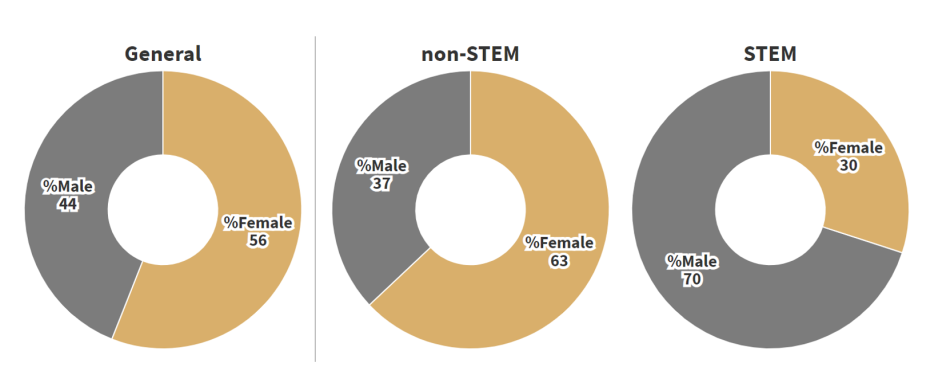
\includegraphics[width=.9\textwidth]{chaps/Images/genderpizza.png}
    \caption{Distribuição de gênero no ensino superior brasileiro}
    \label{fig:genderpizza}
\end{figure}

O projeto SAGA considera a paridade de gênero como aceitável quando varia de 45\% a 55\%. No Brasil, dos 122 cursos superiores de CTEM, apenas 13 deles estão nessa faixa aceitável de paridade de gênero. Considerando as 20 licenciaturas com maior número de alunos matriculados, apenas três delas atingiram a paridade de gênero (Tabela 1). Nesta lista dos 20 melhores cursos, podemos destacar os cursos da área de Tecnologia da Informação como os piores em termos de paridade de gênero, com percentuais de alunas variando de 16\% a uns impressionantes 8\% em Redes de Computadores.

\begin{figure}
    \centering
    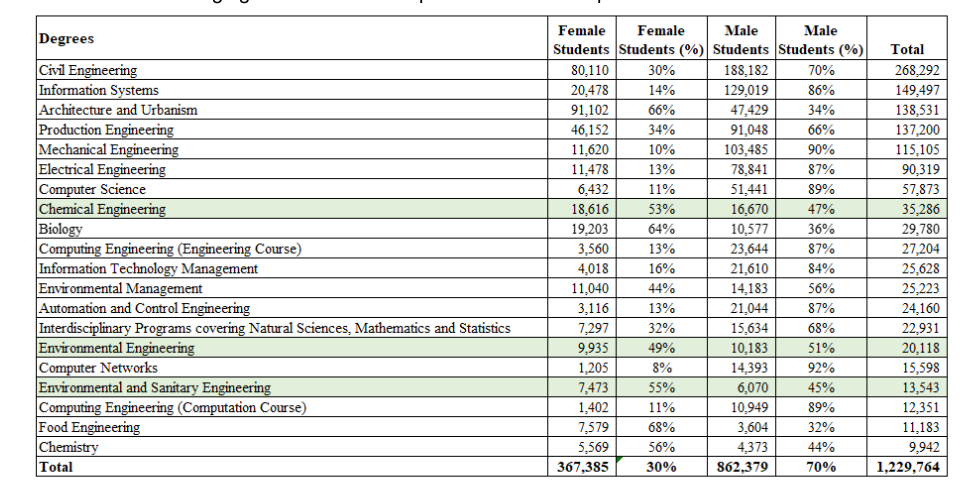
\includegraphics[width=.9\textwidth]{chaps/Images/gendertable.png}
    \caption{Matrículas de gênero no ensino superior brasileiro.}
    \label{fig:gendertable}
\end{figure}

Um dos indicadores sugeridos pela SAGA é o total de professoras por disciplina. Esse indicador é apresentado na Tabela 2 onde se pode verificar que, em termos da proporção total de docentes do sexo feminino em disciplinas relacionadas às CTEM, alcançamos a paridade de gênero no Brasil. Ainda assim, quando olhamos individualmente para as graduações, é possível ver que das 20 disciplinas, apenas quatro têm paridade de gênero com as professoras sendo significativamente sub-representadas em disciplinas como Engenharia, Computação, Física e Astronomia - todas com menos de 30\% de professoras.

\begin{figure}
    \centering
    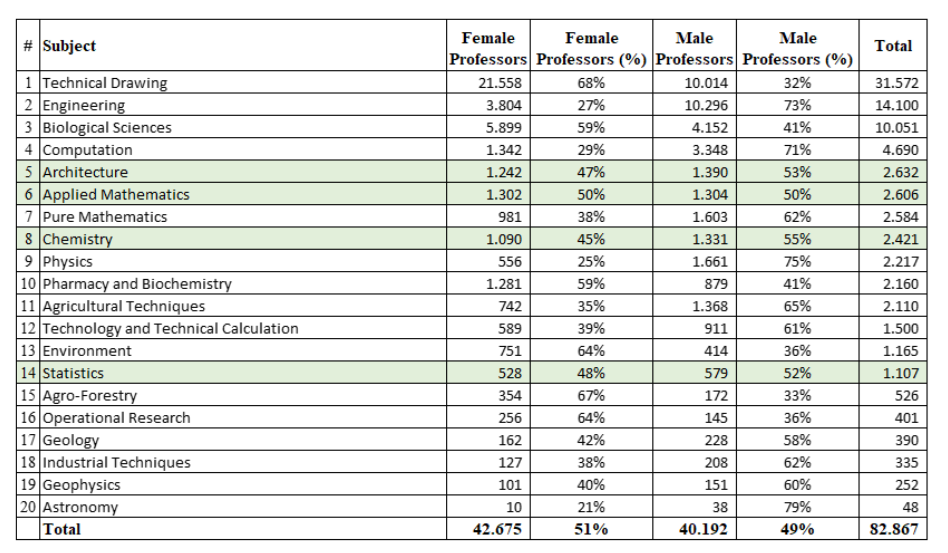
\includegraphics[width=.9\textwidth]{chaps/Images/gendertable2.png}
    \caption{Docentes por disciplina do Ensino Superior Brasileiro.}
    \label{fig:gendertable2}
\end{figure}

\subsection{Iniciativas para Igualdade de Gênero no Brasil}

A Tabela 3 apresenta os resultados de nossa pesquisa de iniciativas para aumentar a igualdade de gênero em STEM no Brasil. Os resultados são apresentados de acordo com o framework fornecido pela SAGA Policy Matrix [18]. Das 25 iniciativas apresentadas, 7 tiveram suas informações cadastradas em nosso formulário online por seus organizadores e 18 foram cadastradas pelos pesquisadores. Como se pode ver, apenas uma iniciativa é organizada pelo governo, enquanto a maioria delas são organizadas ou apoiadas por empresas e universidades. Ao se olhar para o tipo de instrumento, quase todas as iniciativas proporcionam algum tipo de formação em CTEM para mulheres e envolvem a criação e auxílio de pólos tecnológicos, centros de excelência ou comunidades. Apenas duas iniciativas, “Meninas Digitais” e “Para Mulheres na Ciência”, oferecem bolsas de estudo. Além disso, apenas duas iniciativas organizam feiras ou fornecem assistência técnica para mulheres em STEM. o
os beneficiários das iniciativas são, em todos os casos, estudantes e exclusivamente mulheres. A cobertura geográfica das iniciativas é estadual ou nacional, sendo apenas cinco delas internacionais. Os Objetivos de Gênero de Ciência e Tecnologia número 1 da SAGA Unesco se preocupam em mudar as normas sociais e os estereótipos em relação às mulheres em STEM na sociedade. Todas as iniciativas pesquisadas
estão de alguma forma contribuindo com esse objetivo. Outro objetivo da SAGA Unesco que está relacionado com quase todas as iniciativas é o objetivo número 7 que diz respeito à promoção da igualdade de género nas atividades de empreendedorismo e inovação. O objetivo número 3, a participação das mulheres no ensino superior STEM, está relacionado com 20 iniciativas. Já o objetivo menos encontrado nas iniciativas pesquisadas é o objetivo número 6, que trata da igualdade de gênero no processo de formulação de políticas. Em termos de ODS, podemos ver que, como se pode esperar, todos eles estão relacionados ao ODS 5 que se preocupa com o alcance da igualdade de gênero e empoderamento das mulheres. Além disso, 60\% das iniciativas estão de alguma forma relacionadas ao ODS 4, aquele que tem como foco a educação inclusiva e equitativa para todos. Também uma preocupação para um terço das iniciativas pesquisadas é a promoção do crescimento econômico sustentável e do emprego para todos (ODS 8).

\begin{figure}
    \centering
    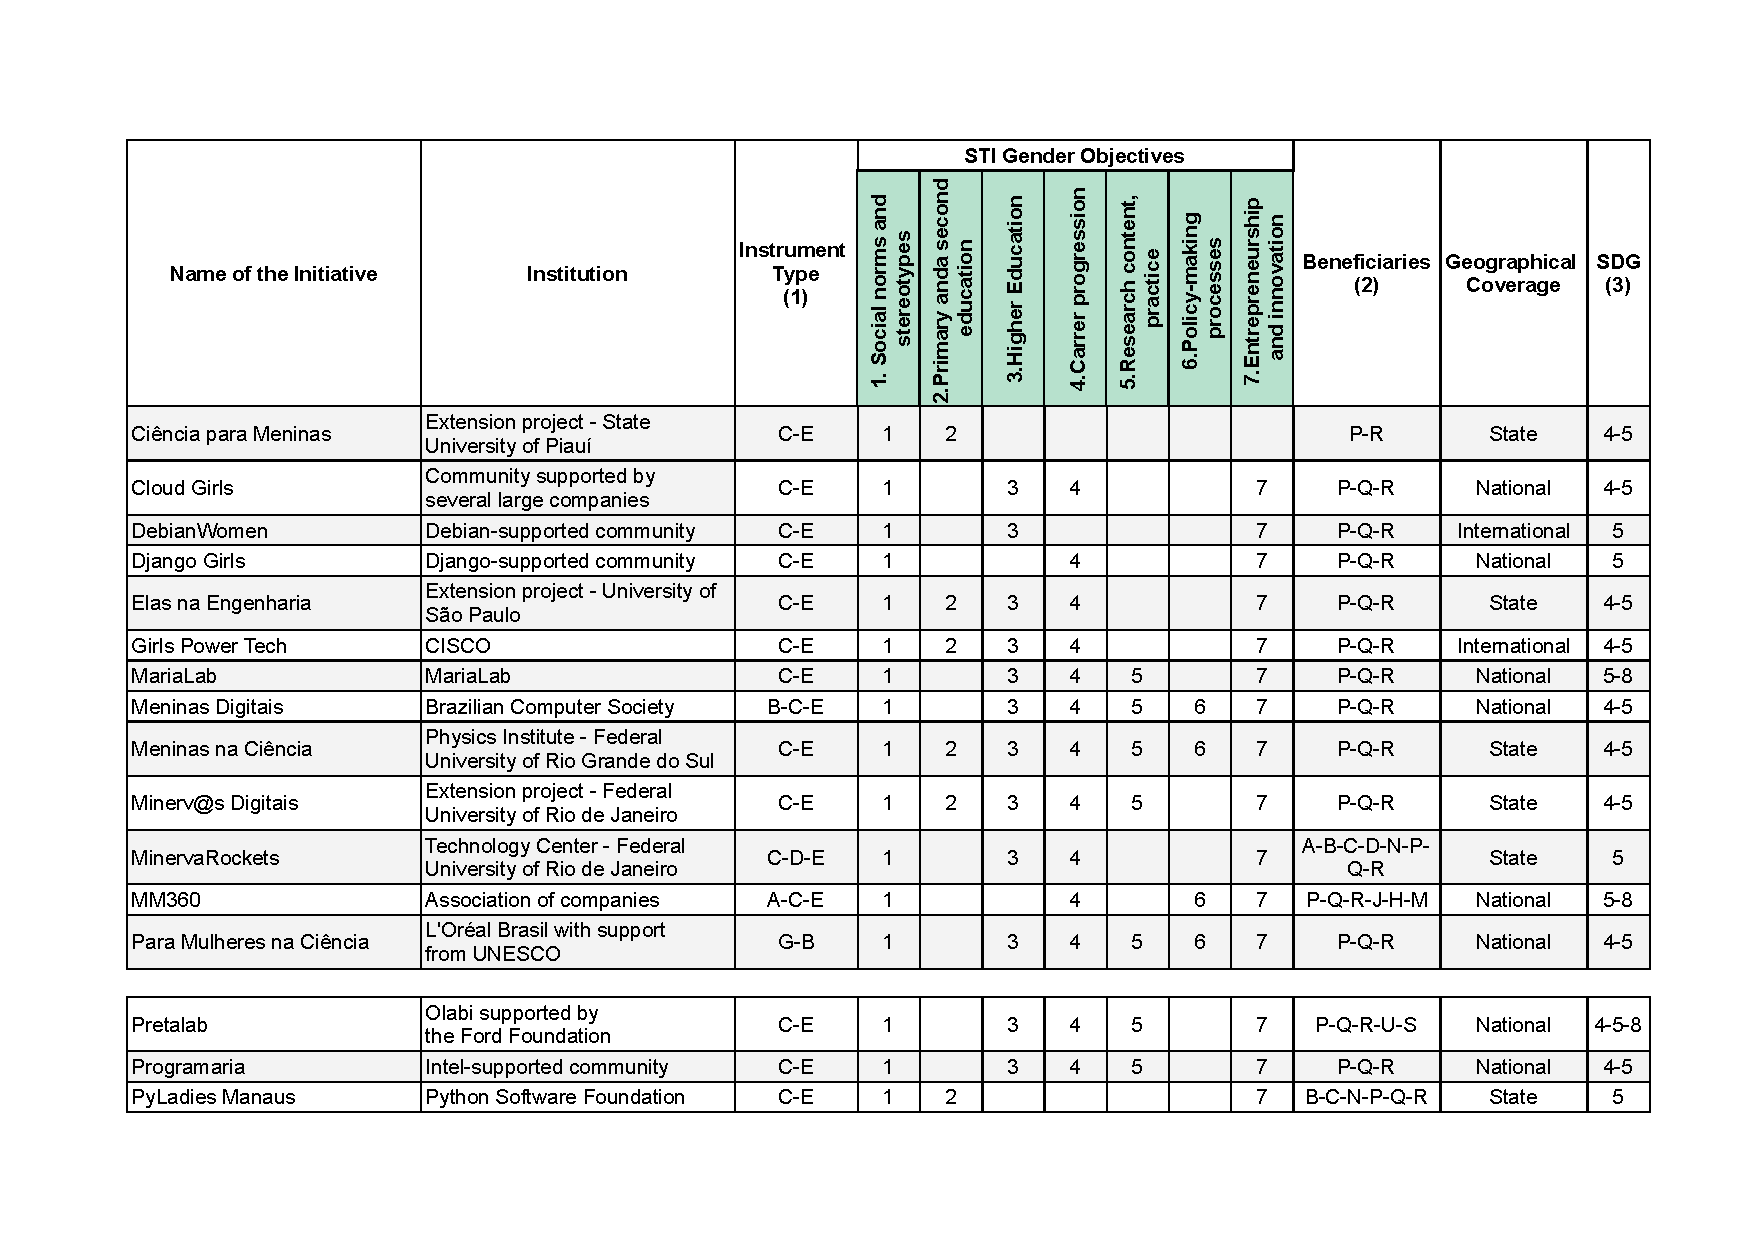
\includegraphics[width=.9\textwidth]{chaps/Images/SAGAMatrixV2.pdf}
    \caption{Iniciativas STEM para a igualdade de gênero no Brasil}
    \label{fig:sagamatriz}
\end{figure}

(1) Tipo de instrumento corresponde às seguintes categorias: A - Assistência Técnica; B - Bolsas / Bolsas de estudo; C - Treinamento; D - Prêmios e Competições; E - Criação e auxílio de pólos tecnológicos, centros de excelência e comunidades; F - Doações (pessoas físicas / jurídicas); G - Feiras; H - confiança; I - Garantia Financeira; J - Incentivos de crédito e capital de risco; K - Incentivos fiscais; L - Empréstimos; M - Serviços de Informação; N - Subsídio (contribuições não reembolsáveis).

(2) Beneficiários ”corresponde às seguintes categorias: A - Centros de pesquisa; B - Universidades; C - Escolas / Faculdades / Institutos; D - Centros de treinamento técnico; E - Institutos públicos; F - Institutos profissionais; G - Organizações STI públicas ou privadas sem fins lucrativos; H - Empresas privadas; I - Pequenas e médias empresas; J - Cooperativas; K - Fundações; L - Grupos locais de P/D; M - associações ad hoc; N - Professores e pesquisadores universitários; O - Equipe técnica e assistentes em STI; P - Alunos; Q - Indivíduos; R - Mulheres (exclusivamente); S - Povos indígenas e comunidades locais; T - Pessoas com deficiência; U - Minorias; V - Profissionais / Ph.D.s.

(3) “Objetivo de Desenvolvimento Sustentável (ODS)” corresponde aos seguintes objetivos: 4 - Garantir uma educação de qualidade inclusiva e equitativa e promover oportunidades de aprendizagem ao longo da vida para todos; 5 - Alcançar a igualdade de gênero e empoderar todas as mulheres e meninas; 8 - Promover o crescimento econômico sustentado, inclusivo e sustentável, emprego pleno e produtivo e trabalho decente para todos.

\subsection{Conclusão}

No Brasil, a Constituição Federal de 1988 garante direitos iguais para homens e mulheres, com especial destaque para o mercado de trabalho. Para que esses direitos sejam efetivamente colocados em termos de igualdade entre homens e mulheres, o caminho para a igualdade de gênero passa por um esforço que depende do governo, ONGs, instituições de ensino e empresas. Particularmente no STEM, esse caminho está sendo mostrado ainda mais difícil de seguir. Além dos desafios enfrentados atualmente pelas mulheres, como a língua predominantemente masculina em ambientes educacionais, de negócios e na cultura em geral, a pandemia COVID-19 cria novos desafios e agrava os anteriormente existentes. A atual pandemia global e o distanciamento social que exige aumentam os obstáculos às mulheres na Ciência, visto que são mais solicitadas no trabalho doméstico e no cuidado, “agravando todas as desvantagens que as mulheres já enfrentam” \citep{scientists_scientist_nodate}. Conforme os dados apresentados por este estudo mostra que existe uma grande lacuna de gênero em STEM, ainda mais em áreas de Tecnologia como Ciência da Computação. Por isso, o Brasil precisa investir em iniciativas exemplares voltadas para a promoção da igualdade de gênero em STEM, como PyLadies (das regiões de Manaus 1, Paraíba 2, Sul de Minas Gerais 3); Meninas na Ciência 4; Ciência para meninas; Elas na Engenharia 5 e Minerva Digitais 6. Essas iniciativas, como mostrado em nossa pesquisa, são importantes para atrair meninas para carreiras em ciência e tecnologia; fomentar o interesse nas áreas exatas e tecnológicas; incentivando e apoiando a participação das mulheres na área tecnológica; incentivando mais meninas e mulheres a aprender sobre a programação; ajudar mais mulheres a se tornarem atuantes em comunidades de software livre; e
incentive as meninas a seguirem carreiras em STEM. Os resultados de nosso estudo podem ser usados para comparar o caso brasileiro com outros países em termos do estado atual da igualdade de gênero no Ensino Superior STEM, bem como as iniciativas para diminuir a lacuna de gênero. O documento também pode ser usado para ajudar os interessados em desenvolver iniciativas para a igualdade de gênero em STEM a entender quais problemas eles querem ajudar a resolver, comparando seus objetivos com os levantados em nosso trabalho.




\subsection{Evento Jornada das Mulheres}

\subsection{Artigos publicados}

\subsection{Trabalhos apresentados}


\section{Motivação de Estudantes}

O conceito de motivação é essencial para a educação. \citep{howard_bell_terrell_1981}, colocou a questão de forma enfática: “Há três coisas a lembrar sobre a educação. O primeiro é a motivação. O segundo é a motivação. A terceira é a motivação ”(\citet{howard_bell_terrell_1981}. Em nosso trabalho, pretendemos identificar os comportamentos relacionados ao aluno, juntamente com um conjunto de características motivacionais, que esperamos que sejam intrínsecas. Saber que a atitude de um aluno durante ela / seu envolvimento com o conteúdo de aprendizagem, dentro ou fora da sala de aula, envolve um relacionamento complexo com várias pessoas, como professores, colegas e equipe, nosso objetivo é envolver o maior número possível de stakeholders no processo de aprendizagem.

\subsection{Teoria da Autodeterminação}

De acordo com \citet{ryan_self-determination_2000}, existem dois aspectos dominantes que podem ser identificados na determinação da motivação: motivação extrínseca e intrínseca.

A motivação intrínseca surgiu na década de 1950 com experimentos em macacos \citet{harlow_learning_1950}. Os primeiros experimentos com humanos foram realizados na década de 1970 \citep{deci_effects_1971} e na década de 1980 aspectos como feedback, prazos e vigilância de motivações intrínsecas foram examinados \citep{deci_intrinsic_1985}.

Com base no conceito anterior de motivação intrínseca, \citet{ryan_self-determination_2017} propôs a Teoria da Autodeterminação (SDT) `` uma teoria organísmica baseada empiricamente do comportamento humano e desenvolvimento da personalidade '' \citep{ryan_self-determination_2017}.

Entre suas características, competência e autonomia, junto com o parentesco, são os principais elementos trabalhados na SDT. Uma vez que os humanos tenham essas necessidades atendidas, a motivação intrínseca pode surgir, e quando elas não são atendidas, a motivação intrínseca é danificada \citet{ryan_self-determination_2017}.

Além disso, essa motivação intrínseca está associada à busca por novidades e desafios, com o intuito de explorar e aprender \citep{ryan_self-determination_2000}, que pode gerar criatividade, desempenho em atividades e uma experiência efetiva \citep{di_domenico_emerging_2017}.

A motivação intrínseca é a forma mais importante de motivação no desempenho do ensino médio  \citep{taylor_self-determination_2014,froiland_intrinsic_2016}, com resultados positivos também no ensino superior  \citep{williams_importance_1998, muller_continuity_2005}, pesquisas incluindo ensino superior e STEM \citep{de_loof_teachers_2019, wang_multilevel_2020} e incluindo ensino superior, STEM e mulheres \citep{moore_connecting_2020, skewes_absent_2018}.

\citep{chua_association_2021} afirma que `` No SDT, o progresso de nosso objetivo é influenciado não apenas pelo que fazemos, mas também pelo que recebemos ". Alguns autores estudam a importância dos objetivos e sua relação com o desempenho dos alunos no contexto da educação \citet{chua_association_2021, benita_emotion_2021, benita_important_2017, benita_when_2014}.

Atualmente, os ambientes de aprendizagem online são importantes mecanismos digitais de atratividade para os alunos, sendo também objetos de pesquisa com a aplicação do SDT \citet{chiu_applying_2021, chiu_digital_2021, chen_motivation_2010}

\subsection{Teoria da Metas}

\section{Autorregulação da Aprendizagem}

\subsection{Mapeamento Sistemático de Autorregulação da Aprendizagem}

Esta seção discute como quizzes são aplicados no campo do aprendizado da engenharia de software e como os quizzes podem ajudar a autorregular o aprendizado do aluno. Para isso, foi realizado um mapeamento sistemático que selecionou os estudos mais relevantes sobre o uso de quizzes na educação, com o objetivo de esclarecer suas relações e impactos mútuos. Nossa análise mostra que o envolvimento do aluno e o trabalho com quizzes são soluções de aprendizagem proeminentes para aumentar a motivação dentro e fora da sala de aula. Argumentamos que compartilhar os quizzes aumentará o potencial para que eles sejam usados como uma ferramenta de autorregulação no ensino de engenharia de software. 

\subsection{Introdução}

A forma de aprendizagem do aluno muda, principalmente com o uso de ferramentas tecnológicas \cite{nilson_creating_2013, fink_creating_2013, ebert_school_2013}. Apesar disso, os tipos de aprendizagem ativa têm como objetivo principal colocar o aluno no centro do processo de aprendizagem e não necessariamente focado no uso da tecnologia. Exemplos disso ocorrem até mesmo nas abordagens utilizadas desde a época de Aristóteles (384 aC-322 aC) \cite{berge_computer_1995}, como uma aula onde os alunos ficam sentados em uma roda, discutindo e refletindo, entre todos, um assunto específico.

Um dos elementos tecnológicos utilizados como recurso de aprendizagem são os quizzes. O uso de quizzes para aprendizagem existem há muitos anos desde que foi discutido pela primeira vez \cite{mawhinney_comparison_1971}. Os quizzes têm sido usados no ensino médio, como uma ferramenta de avaliação e para apoiar outros métodos ou técnicas educacionais em vários campos diferentes, incluindo cursos de engenharia \cite{herold_student_2012, thevathayan_imparting_2017, figueiredo_evaluation_2014}. 

Grimstad \cite {grimstad_are_2004} encontrou resultados que indicam que os alunos podem usar quizzes para melhorar seu desempenho no exame. Para que essa melhoria de desempenho ocorra, Bangert-Drowns \cite {bangert-drowns_instructional_1991} analisou que o feedback está relacionado à aprendizagem e concluiu que os alunos aprendem mais se receberem a resposta correta somente após responder a uma pergunta. Também descobriu que o feedback corretivo é melhor do que simplesmente dizer aos alunos que eles estavam certos ou errados, o que significa que é importante orientar o aluno para as áreas de conteúdo onde ele precisa de revisão ou estudo adicional. Isso se deve ao fato de que, segundo o autor, promove uma estratégia com aspectos de preparação, execução, feedback e autorreflexão.

Para melhor esclarecer o estado atual da pesquisa, envolvendo a utilização de quizzes, na educação e, principalmente, no ensino de Engenharia de Software, realizamos um mapeamento sistemático. Este mapeamento tem como objetivo principal construir uma base de conhecimento que permita explorar quizzes, como ferramenta de aprendizagem autorregulada, no ensino de Engenharia de Software.

Para isso, nosso estudo apresenta as seguintes questões de pesquisa:

\begin {itemize}
    \item\textbf {RQ $ _1 $ - Os quizzes são usados no ensino de engenharia de software?}
     \item\textbf {RQ $ _2 $ - Como os quizzes são usados no ensino de engenharia de software?}
     \item\textbf {RQ $ _3 $ - Os quizzes são usados na educação em engenharia de software para a autorregulação da aprendizagem?}
     \item\textbf {RQ $ _4 $ - Como a aplicação de Quizzes no Ensino de Engenharia de Software pode ser utilizada na Autorregulação da Aprendizagem?}
     \item\textbf {RQ $ _5 $ - Como podemos melhorar o uso de Quizzes no Ensino de Engenharia de Software?}
\end {itemize}

Para responder a essas perguntas, realizamos uma revisão de mapeamento em cinco seções, começando com a introdução (seção 1) e, em seguida, progredindo da seguinte forma: a seção 2 apresenta uma breve revisão dos questionários; A seção 3 inclui os conceitos e metodologia usados neste trabalho; a seção 4 cobre os resultados e nossa análise de pesquisa; E finalmente, na seção 5, nossas conclusões são apresentadas.

\subsection{Educação e Quizzes}

Anderson \cite{anderson_reflections_1984} discutiu e analisou questões sobre processos educacionais. Esses processos incluíam fontes de motivação, como crenças de autoeficácia, gratificação atrasada, atribuições, valores e interesses. Bem como fontes de metacognição como estabelecimento de metas, uso de estratégia, automonitoramento e autoavaliação.

Recentemente, devido aos mais recentes desenvolvimentos em recursos tecnológicos, métodos, dinâmicas e elementos motivacionais, a educação tem transformado os métodos tradicionais de ensino em novos conceitos de aprendizagem, como a sala de aula invertida e a aprendizagem autorregulada.

A sala de aula invertida é uma pedagogia baseada em tecnologia. Bishop e Verleger\cite {bishop_flipped_2013} definem este tipo de aprendizagem como uma instrução individual direta, baseada em computador, fora da sala de aula. Além disso, segundo os autores, esse processo também é realizado por meio de vídeo-aulas e atividades interativas de aprendizagem em grupo em sala de aula.

Como resultado de todas essas transformações na educação, a visão atual da tarefa do aluno na educação mudou para descobrir como aprender novos conhecimentos, em vez de criar verdades e conhecimentos únicos \cite{ebert_school_2013}. Ao refletir sobre suas ações e como encontrar novos conhecimentos, o aluno pode descobrir por si mesmo como superar seus próprios desafios.

Berge\cite{berge_computer_1995} compara a prática da sala de aula invertida com a abordagem baseada no diálogo praticada na Grécia antiga, onde as pessoas aprendiam por meio de desafios e atividades da vida real, compartilhando seus próprios pensamentos e opiniões a fim de encontrar soluções para seus problemas.

Zimmerman e Risemberg \cite{zimmerman_chapter_1997} explicaram as implicações dos diferentes componentes da aprendizagem autorregulada, ressaltando que as tarefas propostas devem permitir que os alunos tomem decisões pessoais e ponderadas com o intuito de regular seus processos de aprendizagem. Com base nessas implicações, o modelo cíclico de Zimmerman \cite{zimmerman_chapter_2000} foi estabelecido (uma representação esquemática está incluída na Fig.\Ref {fig:Zimmerman Model}). De acordo com Zimmerman, a aprendizagem autorregulada visa definir o processo de aprendizagem e as crenças motivacionais de um aluno com base em três fases de autorregulação: Forethought, Performance e Self-Reflection \cite {zimmerman_investigating_2008}.

\begin{figure}[!t]
\centering
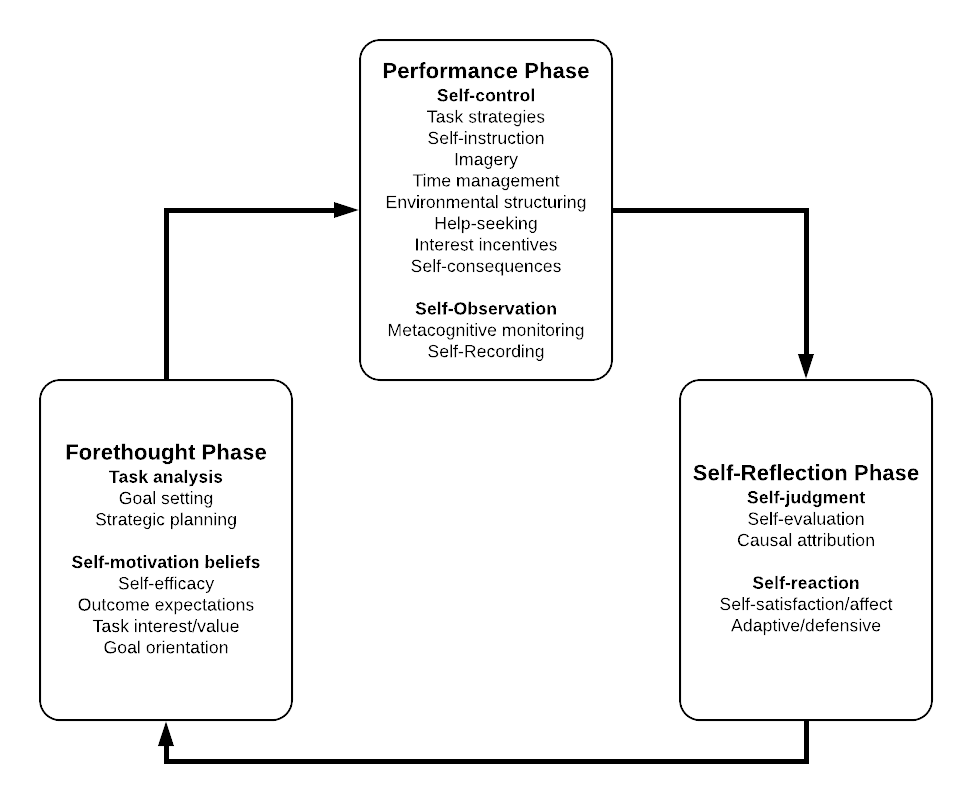
\includegraphics[width=3.5in]{chaps/Images/Zimmerman.png}
\caption{Zimmerman Cyclic Model.}
\label{fig:Zimmerman Model}
\end{figure}

A aprendizagem autorregulada também foi considerada importante nas formas sociais de aprendizagem, como buscar ajuda externa de outras pessoas que não o professor. A questão principal é se o aluno demonstra iniciativa pessoal e capacidade de adaptação. Essas qualidades dos alunos derivam de crenças e sentimentos motivacionais vantajosos \cite{zimmerman_chapter_2000}.

De acordo com Anderson et al. \cite{anderson_taxonomy_2000}, existem dois tipos de avaliação. O primeiro tipo é a avaliação somativa, em que as informações são coletadas pós-aprendizagem para determinar o quão bem o aluno aprendeu o material. O outro tipo é a avaliação formativa, que se preocupa com a coleta de informações sobre o aprendizado e é projetada para melhorar a qualidade ou a quantidade do aprendizado.

Os quizzes são normalmente usados para fazer os testes de avaliação de conhecimentos e habilidades de um aluno. Os quizzes não devem ser entendidos apenas como avaliações sumativas, mas sim como uma experiência de aprendizagem para os alunos, avaliando a eficácia das suas estratégias de estudo e preparação para o teste \cite{nilson_creating_2013}. Como tal, são um dos elementos que podem ser aplicados na educação para melhorar a aprendizagem autorregulada.

É importante considerar que aprender a usar o material de estudo é tão importante quanto aprender o próprio material. Desta forma os alunos irão avaliar suas estratégias e se preocupar com seu desempenho, aprimorando-as adequadamente \cite{fink_creating_2013}. Para tanto, Zimmerman sugere que os alunos devem primeiro ser solicitados a expressar sua confiança na capacidade de resolver um problema antes de começarem a tentar resolvê-lo e reavaliar sua confiança após resolvê-lo. Depois disso, eles devem ser solicitados a escrever uma análise de erros de todos os problemas que eles não resolveram corretamente. Ao fazer a primeira atividade, os alunos aprendem rapidamente a estudar um problema antes de tentar resolvê-lo; enquanto faz o segundo, permite que eles adquiram estratégias de solução de aprendizagem \cite{zimmerman_enhancing_2011}.

Ottenhoff \cite{ottenhoff_learning_2011} afirma que a literatura sobre aprendizagem autorregulada, metacognição e avaliação oferece várias atividades e tarefas que os alunos podem realizar antes, durante e depois dos exames. Algumas atividades e atribuições tornam os alunos mais conscientes do que aprenderam e não aprenderam, enquanto outras atividades envolvem os alunos na avaliação de estratégias de preparação para o teste e no desenvolvimento de estratégias mais eficazes. Todos eles ajudam a melhorar o foco dos alunos em seu aprendizado. De acordo com Nilson \cite{nilson_creating_2013}, os quizzes podem apoiar a aprendizagem autorregulada, fornecendo oportunidades para várias Atividades e Tarefas que ajudam na aprendizagem autorregulada. Incluem Atividades e Tarefas para Preparação para Exames, Atividades Durante um Exame e Atividades e Tarefas Após Exames e Testes.

Antes dos exames, os alunos podem se preparar estudando e melhorando suas áreas de conhecimento mais fracas, mas existem opções que consomem menos tempo. Ao criar perguntas de teste desenvolvidas pelos alunos (de múltipla escolha ou outros tipos de perguntas), os alunos podem revisar o material e avaliar a importância de diferentes partes do material. A criação de uma Folha de Revisão Criada pelo Aluno que mapeia as principais áreas de conteúdo permite ao aluno estimar a porcentagem do exame que será composta por essa área. Esta folha de revisão pode ser melhorada listando o que os alunos acreditam que eles deveriam ser capazes de fazer ou demonstrar e usar esta folha de revisão para se preparar. Os alunos podem elaborar Pesquisas de Conhecimento Pré-exame (quizzes que lhes pedem para avaliar sua confiança em sua capacidade de responder a perguntas ou realizar tarefas relacionadas ao curso). Isso familiariza os alunos com o objetivo do quiz/exame e revela o conteúdo e as áreas de habilidade nas quais eles são fracos ou fortes, permitindo-lhes estreitar o foco de seu estudo e incentivando o estabelecimento de metas e o autoteste.

Durante um exame, os alunos podem ser solicitados a avaliar sua confiança em sua capacidade de resolver um problema antes e depois de resolvê-lo. Incorporar uma pesquisa de conhecimento em um exame pode permitir que os resultados sejam avaliados pela confiança do aluno neles.

Após um Exame, existem várias oportunidades de aprendizagem autorregulada. Pode-se pedir aos alunos que reflitam sobre o quanto estavam preparados para um quiz e sobre a eficácia de seu método de preparação, permitindo-lhes revisar e reconsiderar seus métodos de preparação e capacidade atual. A devolução de um quiz com notas oferece a oportunidade para os alunos resolverem problemas que perderam anteriormente ou resolverem problemas semelhantes. Se isso for combinado com a autoavaliação pré-questionário ou pré-exame de seus níveis de confiança e da eficácia de seu método de estudo, permite saltos impressionantes no aprendizado do aluno. Os alunos podem responder a perguntas no final de um exame para estimar seu desempenho, para descrever sua preparação e para avaliar a dificuldade em diferentes partes do exame. Isso faz com que os alunos reflitam e prevejam seu desempenho, avaliem sua preparação e a eficácia de seus métodos de preparação, reavaliem sua confiança após receberem o exame com notas e vejam se suas estratégias de preparação estão funcionando. A formalização da reavaliação dos métodos e da confiança de um aluno é possível fazendo com que os alunos respondam por escrito a uma série de perguntas depois de verem seu exame com nota, permitindo assim que os alunos desenvolvam um plano de estudo para o próximo exame com base nos resultados do exame anterior. Usando a análise pós-teste, os alunos são capazes de diagnosticar os padrões por trás de seus erros e, assim, obter o tipo de ajuda de que precisam.

Embora existam muitas questões teóricas e práticas sobre como maximizar os benefícios do uso dos quizzes, interromper o aprendizado com perguntas do questionário é benéfico porque pode melhorar o envolvimento do aluno \cite{healy_timing_2017}. Diversas instituições de ensino adotam clickers, que permitem aos instrutores aplicar questionários de múltipla escolha a qualquer momento durante a aula, com feedback imediato para professores e alunos \cite{smith_why_2009}. De acordo com Harley, há um benefício de aprendizagem para os alunos, proporcionado pela ação de testar seus conhecimentos, pela obtenção de feedback e pela natureza interativa do procedimento do clicker. Para os professores, há o benefício da avaliação por ter a capacidade de manter uma avaliação contínua da compreensão dos alunos e prever sua retenção de aprendizagem após a leitura do material \cite{healy_timing_2017}.

Com o entendimento de que os quizzes podem ser aplicados à educação, apesar do aparente desafio e sobrecarga necessários para preparar e administrar questionários em um contexto educacional, este estudo tem como objetivo investigar como os quizzes podem ser benéficos para a aprendizagem autorregulada, no contexto das aulas de engenharia de software.

\subsection{Metodologia}
\label{metodo}

O processo de pesquisa utilizado neste trabalho baseia-se na revisão sistemática da pesquisa de processos em engenharia de software \cite{kitchenham_systematic_2013, kitchenham_systematic_2009} e foi conduzida por meio da plataforma Parsif.al \footnote{https://parsif.al/}.

Nosso processo começou com um mapeamento sistemático que nos permite avaliar e selecionar os estudos mais relevantes sobre o uso de quizzes para auxiliar na autorregulação da aprendizagem. Nossa intenção é identificar a utilização de quizzes na autorregulação da aprendizagem no contexto de alunos de graduação, no ensino de engenharia de software.

Exploramos como o ensino de engenharia de software utiliza quizzes, quais são seus tipos, se é utilizado como ferramenta de autorregulação da aprendizagem e quais resultados positivos e negativos foram encontrados. Para nós, é importante entender como eles podem ser usados de diferentes maneiras. Todos os procedimentos de revisão da literatura - como descrição do que foi planejado, seleção da estratégia, condução da pesquisa e relatório final - são descritos a seguir.

\subsection{Research Planning}
\label{planeja}

Nosso plano de pesquisa foi elaborado contendo: objetivos, questões a responder, busca e seleção, estratégias, avaliação da qualidade e extração de resultados. Nosso planejamento de pesquisa começou com a definição do protocolo para o mapeamento sistemático. Começamos definindo os objetivos de nossa pesquisa:
\begin{itemize}
     \item Analisar publicações científicas que abordem o Ensino de Engenharia de Software;
     \item Analisar publicações científicas que estudam a utilização de Quizzes no Ensino (e em particular como ferramenta pedagógica autorreguladora);
     \item Elaborar uma Revisão e/ou Mapeamento da literatura sobre `` Ensino e Questionários de Engenharia de Software '';
     \item Justificar/motivar a criação/implementação de um repositório de Quiz Compartilhado de Engenharia de Software
\end{itemize}

Nossa próxima etapa foi definir a População, Intervenção, Comparação, Resultado, Contexto (PICOC):
\begin{itemize}
     \item População - `` questionários "
     \item Intervenção - autorregulação da aprendizagem
     \item Comparação - iniciativa OU modelo OU estrutura OU atividades OU métodos OU técnicas
     \item Resultado - apoiar OU melhorar OU otimizar OU ajudar OU ajudar OU especificações
     \item Contexto - Educação em Engenharia de Software
\end{itemize}

Em seguida, definiu-se as questões de pesquisa:
\begin{itemize}
    \item\textbf{RQ $ _1 $ - Os questionários são usados no ensino de engenharia de software?} - O objetivo desta questão é verificar se os questionários são usados como ferramenta de aprendizagem no ensino de engenharia de software.
    
\item\textbf{RQ $ _2 $ - Como os Quizzes são usados no Ensino de Engenharia de Software?} - O objetivo desta questão é entender quais tipos de quizzes foram aplicados e como eles foram usados no Ensino de Engenharia de Software.

\item\textbf{RQ $ _3 $ - Os questionários são usados na Educação em Engenharia de Software para a Autorregulação da Aprendizagem?} - O objetivo desta questão é entender quais áreas de pesquisa, relacionadas à autorregulação da aprendizagem, foram afetadas pelo uso de questionários.

\item\textbf{RQ $ _4 $ - Como a aplicação de Quizzes na Educação em Engenharia de Software pode ser utilizada na Autorregulação da Aprendizagem?} - Esta questão busca identificar quais etapas da autorregulação da aprendizagem, com base no modelo cíclico de Zimmerman, foram aplicados, seus resultados e suas falhas de implementação.

\item\textbf{RQ $ _3 $ - Como podemos melhorar o uso de questionários no ensino de engenharia de software?} - Esta questão busca identificar possíveis melhorias no uso atual de questionários no ensino de engenharia de software.
\end{itemize}.

Em relação às palavras-chave e sinônimos, selecionamos as seguintes palavras-chave, mas optamos por não definir nenhum sinônimo para evitar a obtenção de resultados que escapassem ao escopo deste trabalho:

\begin{itemize}
     \item Quiz
     \item Aprendizagem de Autorregulação
     \item Educação em Engenharia de Software
\end{itemize}

Escolhemos o banco de dados de estudos Scopus \footnote{http://www.scopus.com} como nossa fonte. Para a busca de artigos, utilizamos artigos dos últimos 5 anos em nossas fontes selecionadas. Definimos a seguinte string de pesquisa \emph{`` quiz "AND` `Educação em Engenharia de Software"}.

Definimos vários critérios de inclusão e exclusão para que pudéssemos aceitar ou rejeitar os estudos que obtivemos em nossa busca. Estes são mostrados em \textbf{Tabela\ref{tab:criteria}}.

\begin{table}[ht]
    \centering
        \caption{Critérios de inclusão e exclusão para estudos}
        \begin{tabular}{p{65mm}|p{65mm}}
            \hline
                \textbf{Critérios de inclusão} & \textbf{Critérios de exclusão} \\
            \hline
            \hline
                O estudo apresenta métodos e técnicas possíveis & O estudo aborda questionários fora do contexto da engenharia de software 
                \\
            \hline
                O estudo apresenta possíveis implicações (vantagens e desvantagens)  &
                O estudo é um capítulo de um livro ou editorial \\
            \hline
                O estudo apresenta questões relacionadas à nossa pesquisa  &
                O estudo não está disponível para leitura \\
            \hline
                 - &
                O estudo não está relacionado às questões de pesquisa \\
            \hline
                 - &
                O estudo não foi publicado em inglês \\
            \hline
        \end{tabular}
    \label{tab:criteria}
\end{table}

Após finalizar a definição do protocolo, definimos uma Lista de Verificação de Avaliação da Qualidade que nos permitiu avaliar a qualidade de cada um dos estudos aceitos.

A lista de verificação foi composta por duas questões que consideramos adequadas aos objetivos de nossa pesquisa:

\begin {itemize}
     \item No artigo foram encontrados - Auto-regulação da aprendizagem - afetada pelo uso de quizzes?
     \item No artigo foram encontrados - tipos de quizzes - aplicados no ensino de engenharia de software?
\end{itemize}

Definimos três respostas para as questões e seus respectivos pesos. Eles são mostrados em \textbf {Tabela\ref{tab:scoring_weight}}.

\begin{table}[ht]
    \centering
        \caption{Respostas da pergunta da lista de verificação de avaliação de qualidade e respectivo peso}
        \begin{tabular}{c|c}
            \hline
                \textbf{Responder} & \textbf{Peso} \\
            \hline
            \hline
                Sim & 2.0 \\
            \hline
                Parcial & 1.0 \\
            \hline
                Não & 0.0 \\
            \hline
        \end{tabular}
    \label{tab:scoring_weight}
\end{table}

A pontuação máxima foi calculada automaticamente (4,0) e optamos por um Cutoff Score (que nos permite descartar qualquer estudo que ficasse abaixo da pontuação escolhida) de 3,0.

Para que pudéssemos sistematizar a extração dos dados dos estudos, criamos um Formulário de Extração de Dados que nos ajudaria a encontrar as respostas às nossas dúvidas de pesquisa nos seguintes campos:

\begin{itemize}
    \item \textbf{Tipo de Aplicação de Quizzes} - O objetivo deste campo é extrair dados sobre como os questionários foram aplicados à Engenharia de Software (tipos de questionários). Nos permite responder \textbf{RQ$_1$ - Os quizzes são usados no ensino de engenharia de software?} e \textbf{RQ$_2$ -  Como os quizzes são usados na educação em engenharia de software?}.
    
    \item \textbf{Contexto onde os quizzes foram aplicados} - O objetivo deste campo é extrair dados sobre o contexto onde os quizzes foram aplicados (a que tipo de curso ou sistema os questionários foram aplicados e quando foram aplicados). Isso nos ajudará a encontrar respostas para \textbf{RQ$_1$ - Os quizzes são usados no ensino de engenharia de software?} e \textbf{RQ$_2$ -  Como os quizzes são usados na educação em engenharia de software?}.
    
    \item \textbf{Fases do modelo cíclico de Zimmerman consideradas implícita ou explicitamente} - O objetivo deste campo é extrair dados sobre quais fases do Modelo Cíclico de Zimmerman foram envolvidas ou consideradas no estudo devido à aplicação de questionários. Isso nos ajudará a encontrar respostas para \textbf{RQ$_3$ -  Os quizzes são usados na Educação em Engenharia de Software para a Autorregulação da Aprendizagem?} and \textbf{RQ$_4$ -  Como a aplicação de Quizzes no Ensino de Engenharia de Software pode ser utilizada na Autorregulação da Aprendizagem?}.

    \item\textbf{Tipos de Atividades (Antes, Durante ou Depois do Exame/Questionário) considerada implícita ou explicitamente} - O objetivo deste campo é extrair dados sobre quais tipos de Atividades foram envolvidas ou examinadas no estudo devido à aplicação de questionários. Como o campo anterior, ele nos ajudará a encontrar respostas para \textbf{RQ$_3$ -  Os quizzes são usados na Educação em Engenharia de Software para a Autorregulação da Aprendizagem?} e \textbf{RQ$_4$ -  Como a aplicação de Quizzes no Ensino de Engenharia de Software pode ser utilizada na Autorregulação da Aprendizagem?}.
    
    \item\textbf{Resultados positivos da aplicação de questionários} - O objetivo deste campo é extrair dados sobre quais foram os resultados positivos da aplicação dos Quizzes encontrados pelo estudo. Seremos capazes de olhar para os aspectos positivos da aplicação de quizzes em engenharia de software que podem nos ajudar a raciocinar sobre \textbf{RQ$_5$ -  Como podemos melhorar o uso de quizzes na educação em engenharia de software?}.
    
    \item\textbf{Resultados negativos da aplicação de questionários} -O objetivo deste campo é extrair dados sobre quais foram os resultados negativos da aplicação dos Quizzes encontrados pelo estudo. Por estarmos cientes dos aspectos negativos, podemos tentar minimizá-los para responder \textbf{RQ$_5$ -  Como podemos melhorar o uso de quizzes na educação em engenharia de software?}.
\end{itemize}.

\subsection{Conduzindo a Pesquisa}

A seleção dos estudos utilizou um procedimento de filtragem em duas etapas: a primeira etapa envolveu a leitura dos estudos e filtrá-los de acordo com se um estudo individual está relacionado à nossa pesquisa; enquanto a segunda etapa envolveu um sistema de pontuação, em que os estudos pré-selecionados da etapa anterior foram analisados detalhadamente para determinar o grau de resposta à pesquisa (ou seja: total, parcialmente ou não todos). Em seguida, a extração foi realizada consolidando as informações relevantes contidas nos estudos. Por fim, foi realizada uma análise do resultado da etapa anterior para que pudéssemos responder às questões de pesquisa.

A pesquisa que conduzimos teve as seguintes etapas em ordem:
\begin{enumerate}

    \item \emph{Search} - Nesta etapa, pesquisamos os repositórios selecionados para a string de pesquisa definida anteriormente. Isso nos permite obter uma lista de estudos que correspondem à nossa string de pesquisa, que usaremos na próxima etapa.

    \item \emph{Import Studies} - Esta etapa permite importar as meta-informações dos estudos (resumo, autores, data, etc.) para manter um banco de dados para gerenciar as próximas etapas.

    \item \emph{Study Selection} - Durante esta etapa, aceitamos ou rejeitamos os estudos em nosso banco de dados de acordo com os critérios que definimos durante o planejamento.

    \item \emph{Quality Assessment} - Aqui, aplicamos a Lista de Verificação de Avaliação de Qualidade previamente definida aos estudos de nosso banco de dados que foram aceitos na etapa de Seleção de Estudos para pontuá-los individualmente.

    \item \emph{Data Extraction} - Usamos o Formulário de Extração de Dados criado anteriormente para extrair os dados relevantes para nossa pesquisa dos estudos em nosso banco de dados que pontuaram acima de 3,0 na etapa anterior.
    

    \item \emph{Data Analysis} - Analisamos os dados que resultaram da aplicação de nossa metodologia de pesquisa.
\end{enumerate}

\subsection{Resultados}

Nesta seção, os resultados da revisão são apresentados e analisados.

\subsection{Search}
A execução de nossa consulta de pesquisa retornou um total de 68 estudos, dos quais tínhamos 0 duplicatas.

\subsection{Study Selection}
Nossa análise dos estudos obtidos durante a Pesquisa nos fez rejeitar 46 estudos porque eles não eram relevantes para as nossas questões de pesquisa.

\subsection{Quality Assessment}
Em seguida, pontuamos os 22 estudos restantes usando a Lista de verificação de avaliação de qualidade definida anteriormente, o que resultou na manutenção dos 13 estudos. Uma visão geral dos resultados pode ser mostrada em \textbf{Table\ref{tab:quality_assessment}}.

\begin{table}[ht]
    \centering
        \caption{Visão geral das pontuações de avaliação da qualidade dos estudos}
        \begin{tabular}{c|c}
            \hline
                \textbf{Score} & \textbf{Número de estudos} \\
            \hline
            \hline
                0 & 
                1 \\
            \hline
                1 & 
                2 \\
            \hline
                2 & 
                6 \\
            \hline
                3 & 
                1 \\
            \hline
                4 & 
                12 \\
            \hline
        \end{tabular}
    \label{tab:quality_assessment}
\end{table}

\subsection{Data Extraction}

Em nossa revisão, obtivemos informações relevantes sobre quizzes em cursos de engenharia de software \cite{figueiredo_evaluation_2014}, bem como revisões sistemáticas de trabalhos que aplicaram questionários neste contexto educacional, tais como \cite{luxton-reilly_introductory_2018} e \cite {crow_intelligent_2018} . Também encontramos estudos que avaliam resultados em um ambiente de sala de aula invertida que trabalha com aprendizagem autorregulada, como \cite{ogawa_evaluation_2018} e \cite{herold_student_2012}. Práticas de aprendizagem dos alunos, como \cite{thevathayan_imparting_2017} e \cite{verdu_distributed_2012}. Um desses estudos, \cite{wu_improvement_2011} apresentou uma proposta para um conceito de jogo de aula que pode melhorar a comunicação e motivar os alunos por meio de aulas mais interessantes e sem descrever claramente como os alunos podem melhorar sua autorregulação da aprendizagem em sala de aula, este estudo pode fornecer questões importantes sobre a motivação dos alunos para autorregulação da aprendizagem  e o interesse pelo jogo, neste caso um jogo de perguntas multiplayer chamado Lecture Quiz.

\textbf{Table \ref{tab:quizzes_application_types}} mostra os dados extraídos relacionados ao \textbf{Tipo de Aplicação de Quizzes}.

\begin{table}[ht]
    \centering
        \caption{Tipos de aplicação de quizzes}
        \begin{tabular}{c|c|c}
            \hline
                \textbf{Tipos de aplicação de quizzes} & \textbf{Número de Estudos}  & \textbf{Estudos} \\
            \hline
            \hline
                Quiz Games & 
                4 &
                \cite{petri_quality_2017, petri_games_2018, verdu_distributed_2012, wu_improvement_2011} \\
            \hline
                Online Quizzes & 
                4 & 
                \cite{figueiredo_evaluation_2014, coore_facilitating_2019, luxton-reilly_introductory_2018, krugel_computational_2017} \\
            \hline
                Pop-Quizzes & 
                1 &
                \cite{luxton-reilly_introductory_2018} \\
            \hline
                Gamified Quizzes & 
                1 & 
                \cite{luxton-reilly_introductory_2018} \\
            \hline
                Quiz Creation & 
                1 & 
                \cite{ogawa_evaluation_2018} \\
            \hline
                Generic Quizzes & 
                5 & 
                \cite{crow_intelligent_2018, ogawa_evaluation_2018, acharya_infusing_2017, thevathayan_imparting_2017, herold_student_2012} \\
            \hline
        \end{tabular}
    \label{tab:quizzes_application_types}
\end{table}

Encontramos uma variedade de \textbf{Contextos onde os quizzes foram aplicados}. Separamos esses contextos nas seguintes categorias: \textbf{In-Lecture vs Outside-Lecture} e \textbf{Tipo de Curso} (Tradicional, Online, Híbrido ou Sistema Tutor Inteligente). \textbf{Tabela\ref{tab:context_in_vs_out}} mostra os contextos \textbf {In-Lecture vs Outside-Lecture} que foram encontrados para a aplicação de questionários.

\begin{table}[ht]
    \centering
        \caption{Contextos em que os quizzes foram aplicados: na aula x fora da aula}
        \begin{tabular}{c|c|c}
            \hline
                \textbf{In-Lecture vs Outside-Lecture} & \textbf{Number of Studies}  & \textbf{Studies} \\
            \hline
            \hline
                In-Lecture Quizzes &
                6 &
                \cite{petri_quality_2017, crow_intelligent_2018, acharya_infusing_2017, krugel_computational_2017, thevathayan_imparting_2017, wu_improvement_2011} \\
            \hline
                Outside-Lecture Quizzes &
                7 &
                \cite{figueiredo_evaluation_2014, coore_facilitating_2019, luxton-reilly_introductory_2018, ogawa_evaluation_2018, thevathayan_imparting_2017, herold_student_2012, verdu_distributed_2012} \\
            \hline
        \end{tabular}
    \label{tab:context_in_vs_out}
\end{table}

\textbf{Table \ref{tab:context_course_type}} mostra o \textbf{Type of Course} contextos que foram encontrados para a aplicação de quizzes.

\begin{table}[ht]
    \centering
        \caption{Contextos em que os quizzes foram aplicados: Tipo de curso}
        \begin{tabular}{c|c|c}
            \hline
                \textbf{Type of Course} & \textbf{Number of Studies}  & \textbf{Studies} \\
            \hline
            \hline
                Traditional Courses &
                6 & 
                \cite{petri_quality_2017, coore_facilitating_2019, luxton-reilly_introductory_2018, acharya_infusing_2017, thevathayan_imparting_2017, wu_improvement_2011} \\
            \hline
                Online Courses &
                4 &
                \cite{figueiredo_evaluation_2014, ogawa_evaluation_2018, krugel_computational_2017, verdu_distributed_2012} \\
            \hline
            Online Courses
                Hybrid Course &
                1 &
                \cite{figueiredo_evaluation_2014} \\
            \hline
                Intelligent Tutor System &
                2 &
                \cite{crow_intelligent_2018, thevathayan_imparting_2017} \\
            \hline
                Inverted Class Course &
                3 &
                \cite{ogawa_evaluation_2018, herold_student_2012, coore_facilitating_2019} \\
            \hline
        \end{tabular}
    \label{tab:context_course_type}
\end{table}

Em relação a \textbf{Fases do Modelo Cíclico de Zimmerman (implícita ou explicitamente) consideradas}, os artigos não analisaram questionários diretamente pela perspectiva do Modelo Cíclico de Zimmerman, mas os abordaram mesmo assim. \textbf{Table \ref{tab:zimmerman_phase}} mostra os resultados.

\begin{table}[ht]
    \centering
        \caption{Fases do modelo cíclico de Zimmerman consideradas implícita ou explicitamente}
        \begin{tabular}{c|c|c}
            \hline
                \textbf{Phase} & \textbf{Number of Studies}  & \textbf{Studies} \\
            \hline
            \hline
                Forethought &
                6 &
                \cite{coore_facilitating_2019, luxton-reilly_introductory_2018, krugel_computational_2017, herold_student_2012, verdu_distributed_2012, wu_improvement_2011} \\
            \hline
                Performance &
                6 & 
                \cite{petri_quality_2017, coore_facilitating_2019, luxton-reilly_introductory_2018, ogawa_evaluation_2018, krugel_computational_2017, verdu_distributed_2012} \\
            \hline
                Self-Reflection &
                6 &
                \cite{petri_quality_2017, figueiredo_evaluation_2014, coore_facilitating_2019, luxton-reilly_introductory_2018, krugel_computational_2017, thevathayan_imparting_2017} \\
            \hline
        \end{tabular}
    \label{tab:zimmerman_phase}
\end{table}

Fases do modelo cíclico de Zimmerman consideradas implícita ou explicitamente \textbf{Types of Activities}. Os resultados são mostrados em \textbf{Table \ref{tab:activities_types}}.

\begin{table}[ht]
    \centering
        \caption{Tipo de atividades (antes, durante ou depois do exame / questionário) considerada implícita ou explicitamente}
        \begin{tabular}{c|c|c}
            \hline
                \textbf{Activity Type} & \textbf{Number of Studies}  & \textbf{Studies} \\
            \hline
            \hline
                Activities Before an Exam &
                7 & 
                \cite{figueiredo_evaluation_2014, coore_facilitating_2019, luxton-reilly_introductory_2018, ogawa_evaluation_2018, herold_student_2012, verdu_distributed_2012, wu_improvement_2011} \\
            \hline
                Activities During an Exam &
                1  &
                \cite{verdu_distributed_2012} \\
            \hline
                Activities After an Exam &
                6 &
                \cite{petri_quality_2017, figueiredo_evaluation_2014, coore_facilitating_2019, luxton-reilly_introductory_2018, krugel_computational_2017, thevathayan_imparting_2017} \\
            \hline
        \end{tabular}
    \label{tab:activities_types}
\end{table}

Os estudos mostraram os seguintes \textbf{Resultados Positivos da Aplicação de Quizzes}: Jogos Educativos Contribuem Positivamente para a Experiência de Aprendizagem \cite{petri_quality_2017}, 
Os questionários permitem uma melhor autoavaliação \cite{figueiredo_evaluation_2014},
Os Pop-Quizzes melhoram o desempenho dos alunos e os Gamified Quizzes melhoram o envolvimento dos alunos \cite{luxton-reilly_introductory_2018},
Os questionários e a criação de questionários aumentaram o desempenho da tarefa \cite{ogawa_evaluation_2018},
Os Quiz Games podem promover uma experiência envolvente para os jogadores \cite{petri_games_2018}.
Os usuários gostaram da interatividade fornecida pelos questionários online, \cite{krugel_computational_2017}.
Os questionários que permitem o diagnóstico de erros comuns permitem que os alunos melhorem, e a classificação das questões do questionário em conceitos e níveis cognitivos permite que a equipe do curso e os alunos identifiquem áreas problemáticas \cite{thevathayan_imparting_2017},
Os questionários foram eficazes como um motivador para assistir a palestras em uma sala de aula invertida \cite{herold_student_2012},
Os Quiz Games melhoraram os resultados acadêmicos dos alunos \cite{verdu_distributed_2012}, e os Jogos de Quiz In-Lecture fizeram os alunos prestar mais atenção e tiveram um efeito positivo na aprendizagem \cite{wu_improvement_2011}.
Encontramos aspectos motivacionais na aprendizagem que foram aplicados em alguns trabalhos como forma de melhorar a aprendizagem, incluindo a aprendizagem ativa, relatados por \cite{figueiredo_evaluation_2014, petri_quality_2017, acharya_infusing_2017, herold_student_2012, petri_games_2018}. Como forma de gerar feedback dos alunos, foi citado por \cite{figueiredo_evaluation_2014, krugel_computational_2017, verdu_distributed_2012}, o envolvimento do aluno, incluindo a motivação, foi encontrado em \cite{coore_facilitating_2019, luxton-reilly_introductory_2018,verdu_distributed_2012}. Além disso, foi encontrado trabalho para melhorar a atitude do aluno \cite{luxton-reilly_introductory_2018}, melhorar a experiência do aluno em \cite{luxton-reilly_introductory_2018, petri_games_2018}, melhorar a satisfação do aluno em \cite{verdu_distributed_2012} e melhorar a comunicação do aluno em \cite{wu_improvement_2011}.

Os \textbf{resultados negativos da aplicação de questionários} destacados pelos estudos foram os seguintes: Os quizzes de preparação antes da aula não tiveram nenhum benefício \cite{luxton-reilly_introductory_2018}, e
Testes semanais avaliados podem aumentar a ansiedade dos alunos \cite{herold_student_2012}.

\subsection{Análise de dados}

Após sintetizar os dados extraídos, respondemos às nossas perguntas de pesquisa:

\textbf{RQ $ _1 $ - Os questionários são usados no ensino de engenharia de software?} -
Podemos responder a essa pergunta claramente com um sim. Os questionários são usados no ensino de engenharia de software.

\textbf{RQ $ _2 $ - Como os questionários são usados no ensino de engenharia de software?} -
Os questionários podem ser aplicados de várias formas. Descobrimos que eles podem ser aplicados como Quizzes Genéricos, como Quizzes Online, como Pop-Quizzes, como Quizzes Gamificados, em Quiz Games ou, alternativamente, como um exercício na criação de Quizzes. Os contextos em que os vimos sendo aplicados também foram variados e encontramos 2 dimensões importantes para o contexto: onde foram aplicados em aula ou fora de aula, e em que tipo de curso / sistema de aprendizagem foram aplicados (tradicional, online, Sistema Tutor Híbrido ou Inteligente).

\textbf{RQ $ _3 $ - Os questionários são usados na Educação em Engenharia de Software para a Autorregulação da Aprendizagem?} - Os dados nos dizem que sim, os questionários são usados na Educação em Engenharia de Software como uma aprendizagem autorregulada. Nos estudos, encontramos exemplos que abordaram ou enfocaram cada uma das diferentes fases do Modelo Cíclico de Zimmerman. Além disso, no que diz respeito às Atividades de aprendizagem autorregulada apoiadas por questionários, vimos que foram encontrados todos os tipos de atividades de aprendizagem autorregulada que os questionários apoiam, mesmo que o fizessem de forma implícita e não explícita.

\textbf{RQ $ _4 $ - Como a aplicação de Quizzes no Ensino de Engenharia de Software pode ser utilizada na Autorregulação da Aprendizagem?} - Os dados extraídos mostram que ela pode ser utilizada para dar suporte a diferentes fases do Modelo Cíclico de Zimmerman, e diferentes tipos de atividades de aprendizagem autorreguladas. No entanto, conforme mencionado anteriormente, isso foi feito implicitamente na maioria dos casos e não explicitamente.

\textbf{RQ $ _5 $ - Como podemos melhorar o uso de Quizzes no Ensino de Engenharia de Software?} - Não encontramos uma resposta clara para esta questão. Os estudos examinados mostraram alguns aspectos negativos que precisam ser levados em consideração cuidadosamente ao usar questionários. Precisamos ter certeza de que a aplicação dos questionários não aumenta a ansiedade do aluno e também precisamos examinar cuidadosamente como aplicar os questionários de preparação para que possam produzir os benefícios adequados. Também é importante considerar como maximizar os benefícios para o desempenho do aluno, engajamento, motivação, atitude, os benefícios de ter um mecanismo de feedback e os benefícios de usá-los como uma ferramenta de autoavaliação e diagnóstico. Uma resposta provisória, mas sem suporte para esta pergunta, pode simplesmente ser, facilitar os questionários de aplicativos para o ensino de engenharia de software. Isso pode ser obtido por meio de um repositório compartilhado de questionários para que possam ser facilmente implantados. Essa ideia pode ser expandida ainda mais, fornecendo as ferramentas necessárias para gerenciar e administrar esses questionários. Uma limitação que encontramos nos estudos foi que eles não abordaram explicitamente o Modelo Cíclico de Zimmerman e as já mencionadas Atividades Apoiadas por Questionários. Suspeitamos que uma implantação de Quizzes na Educação em Engenharia de Software que aborda ou enfoca esses aspectos explicitamente pode obter resultados positivos mais fortes e possivelmente minimizar os negativos.

\subsection{Conclusão}

Esta seção examinou o impacto dos quizzes na aprendizagem autorregulada a fim de identificar as melhores aplicações dos questionários no campo da engenharia de software e, para isso, mapeamos e analisamos trabalhos recentes. A revisão usou uma abordagem estruturada com etapas bem definidas. Alguns estudos passaram por etapas de filtragem antes de serem aprovados para análises posteriores. Os resultados da análise mostraram os benefícios potenciais do uso de questionários como uma ferramenta para a aprendizagem autorregulada.

Assim, encontramos nestes estudos desafios comuns e propostos para abordar a utilização de quizzes no contexto da engenharia de software e para melhorar a aprendizagem autorregulada dos alunos. Também foi possível identificar falhas, principalmente relacionadas à correta aplicação do modelo cíclico de Zimmerman, que fornece a base e o processo de suporte à aprendizagem autorregulada dos alunos. Esta relação entre aprendizagem e motivação tem um grande impacto nos ambientes educacionais, e como consequência, podemos dizer que os quizzes podem ser utilizados como forma de avaliação dos alunos, mas também para estimular a participação, motivação e aprendizagem destes alunos. Acreditamos que os estudos atuais podem ser mais bem explorados e com mais pesquisas nesta área, principalmente no que se refere a:

\begin{itemize}
    \item Modelos auto-reguladores, métodos e técnicas de aprendizagem apoiados no uso de quizzes
    \item Pesquisa relativa ao impacto, na forma de aprendizagem, na engenharia de software
    \item Uso de quizzes compartilhados entre várias instituições
    \item Procedimentos para avaliar a qualidade e validade das perguntas do questionário com base em critérios científicos
\end{itemize}

Argumentamos que, devido aos benefícios anteriormente referidos e devido ao esforço de bootstrapping necessário para criar, revisar e usar quizzes, um corpo padrão de perguntas e respostas revisadas por pares que podem ser reutilizadas em diferentes faculdades que podem refletir melhor o estado da arte e conhecimentos atuais sobre o tema a ser ministrado. Pode ser uma contribuição útil para o ensino de engenharia de software, por conferir a capacidade de potencialmente analisar as habilidades dos alunos em várias universidades, o que pode permitir que os professores entendam melhor as fragilidades do currículo e as áreas problemáticas que podem causar problemas para os alunos, como além de fornecer uma melhor compreensão de quais são esses problemas.


\section{Learning Management Systems(LMS)}

\subsection{MOOCS}


\section{Narrativa}

\subsection{O poder das histórias, personagens e modelos de comportamento na educação}

Nesta seção, discutimos como as histórias são importantes, especialmente na educação, e como os personagens e modelos de comportamento são influenciadores da motivação. Além disso, faremos uma revisão das definições de narrativas e buscaremos compreender como esses elementos, juntos, impactam positivamente a educação STEM para mulheres, transformando seus medos em força. Mais adiante, criaremos uma história baseada em um modelo narrativo de 12 etapas, a Heroine’s Learning Journey, organizada em 3 atos, que incluem vídeos motivacionais e imagens contendo exemplos de mulheres de sucesso nas áreas de STEM. Além disso, usaremos personagens, como Atenas, para motivar jovens estudantes durante o curso de STEM.

As histórias estão por toda parte. Ouvimos, lemos, escrevemos e contamos histórias \citep{alterio_learning_2016} para motivar, transmitir informações e partilhar experiências, estimulando a nossa imaginação e melhorando a nossa memória \citep{alterio_learning_2016}.

Uma vez que as histórias estimulam a nossa imaginação, podemos reconhecer que contar histórias pode, em certas condições, provocar uma mudança na forma como entendemos os fatos \citep{alterio_learning_2016}. A condição para tais mudanças está relacionada à forma como contamos a história.

\citet{davis_engaging_2007} afirmam que as histórias constituem a base da experiência educativa, exemplificando a eficácia do ensino há muitos anos, que incorporou o saber factual em imagens e narrativas ricas. Entre os novos desafios agora presentes na educação, \citet{bruner_life_2004} vê as narrativas como uma forma de criar um mundo em função da mente, não como uma descrição de fenômenos objetivos.
Essa forma de entender a narrativa, segundo o autor, oferece uma possibilidade educacional transformadora: o criador como agente de sua própria mudança e aprendizagem \citep{bruner_life_2004}.

\citet{broom_becoming_2021}, usando ressonância magnética funcional, encontrou evidências de que quando as pessoas se identificam com o personagem de uma história, são influenciadas a assumir algumas de suas características.
Eles também descobriram que quanto mais as pessoas estão imersas na narrativa, mais elas tendem a se "tornar" o personagem fictício, usando a parte do cérebro responsável por pensar sobre si mesmas.

Portanto, a identificação com um personagem fictício pode levar a mudanças nas crenças, atitudes e comportamentos dos indivíduos \citep{oatley_meetings_1999}.

Por exemplo, muitos educadores já relataram que se sentiram inspirados por personagens, como o personagem de Robin Williams, John Keating, em `` Dead Poets Society '' \citep{noauthor_real_2014} e que isso mudou a forma como eles veem o processo educacional. Por outro lado, várias mulheres relataram ter sido influenciadas a seguir carreira na área da saúde devido ao papel de Meredith Gray, interpretada pela atriz Ellen Pompeo na série de TV Grays Anatomy \citep{news_greys_2017}.

Os modelos femininos também influenciam as mulheres a ingressar na carreira STEM \citep{cheryan_female_2011, corbett_solving_2015}. Além disso, a leitura de biografias de mulheres bem-sucedidas em áreas STEM melhora as percepções das mulheres sobre STEM \citep{shin_effects_2016} e também ajuda as mulheres a persistirem em cursos STEM \citep{herrmann_effects_2016}.

Howard Gardner acredita em múltiplas abordagens para entender \citep{gardner_disciplined_2021}. Uma forma de envolver o aluno e colocá-lo no centro do tópico é a narrativa. Na visão de Gardner, a narrativa tem protagonistas, conflitos, problemas a serem resolvidos, metas a serem alcançadas, tensões suscitadas e, muitas vezes, amenizadas. `` O ponto de entrada da narrativa se dirige aos alunos que gostam de aprender sobre tópicos por meio de histórias "\citep{illeris_multiple_2018}.

\subsection{Estruturas narrativas}

A noção de uma estrutura narrativa foi conceituada na antiguidade por filósofos gregos como Aristóteles e Platão\citep {page_new_2011}. Na tradição aristotélica, a narrativa é entendida como representação e não como imitação \citep{hamburger_logic_1973}. Aristóteles propôs uma estrutura de três atos para a narrativa \citep{brutsch_three-act_2015, wedin_aristotles_2000}, que foi estudada e aprimorada ao longo do tempo. Esses três atos são comumente referidos como Configuração, Conflito e Resolução.

\citet{prince_narratology_1982} definiu narrativa como `` a representação de pelo menos dois eventos reais ou fictícios em uma sequência de tempo, onde nenhum pressiona ou provoca o outro '' e \citeauthor{cohn_transparent_1984}, recentemente declarou que a narrativa é `` uma série de declarações que tratam de uma sequência causalmente relacionada de eventos que afetam os seres humanos (ou semelhantes aos humanos) '' \citep{cohn_distinction_2000}.

Desse modo, podemos observar que o estudo da sociedade é uma narrativa, com maior potencial de transformações culturais. É por meio de suposições e crenças que construímos essas narrativas e contamos a história.

Mark Tennant é o autor de The Learning Self \citep{tennant_learning_2012}. A Tennant acredita na compreensão do autodesenvolvimento e que a biografia, a narrativa e a história de vida estão ligadas à pesquisa acadêmica, ao ensino e à cultura popular. Na visão de Tennat, o poder de transformação pessoal está ligado a si mesmo e ao mundo ao redor da pessoa, onde as narrativas desempenham um papel fundamental `` As pessoas, ao que parece, têm um apetite insaciável de se expressar através de narrativas biográficas e explorar as narrativas dos outros em comparação com as suas próprias '' \citep{illeris_life_2018}. As narrativas de grandes personalidades podem transformar nossa forma de pensar, nos fazer refletir e adquirir autodeterminação. Usando a história do Imperador Adriano como exemplo, o autor afirma que as narrativas das nossas histórias de vida estão relacionadas com o nosso estado emocional, as nossas relações interpessoais e sociais \citep{illeris_life_2018}.

São muitas as narrativas para personagens, interesses e ideologias distintas, e seu poder está diretamente ligado ao número de pessoas que são influenciadas por uma determinada história, nas quais se identificam.

\citet{hamburger_logic_1973} acredita que a representação da vida dos personagens pode ser o elo entre a ficção e a realidade.
Com base nessa premissa, \citeauthor{hamburger_logic_1973} afirma que existem padrões de linguagens exclusivas na ficção e esses padrões são condutores da atividade mental, verbos da consciência, monólogos interiores e narrados, advérbios temporais e espaciais referentes a personagens aqui e agora.
\citet{cohn_transparent_1984} analisa os conceitos de \citeauthor{hamburger_logic_1973} e os traduz como `` A ficção narrativa é o único gênero de alfabetização, bem como o único tipo de narrativa, em que os pensamentos não ditos, sentimentos e percepções de uma pessoa além do orador pode ser retratado ''

Hoje em dia, segundo \citet{richardson_recent_2000}, ``A narrativa está em todo lugar''. Teologia narrativa, tratamentos psicológicos por meio de terapia narrativa e construção de narrativas para apoiar grupos minoritários, são exemplos da importância da narrativa na pesquisa. A narrativa é considerada o "veículo básico do conhecimento humano" \citep{richardson_recent_2000}.

A partir da década de 1990, surgiram novas demandas que influenciam a forma como as narrativas são interpretadas e aplicadas. \citet{aarseth_cybertext_1997} identificou novos desafios e afirma que as demandas radicais por uma revolução narrativa surgiram à luz do hipertexto e dos jogos. Mais adiante, um novo tipo de interdisciplinaridade começa a emergir, como desenvolvimentos na teoria da inteligência artificial, estudos de hipertexto e avanços nas ciências cognitivas aplicadas à teoria narrativa \citep{richardson_recent_2000}.

Dentre esses novos desafios e transformações no campo da narrativa, novos conceitos surgiram, juntamente com questões sobre como as histórias são produzidas e vividas, e também discutidas, por exemplo, em relação à sua interatividade e imersão \citep{page_new_2011}.

\citet{page_new_2011}, que aborda o tema dos hipertextos em forma de narrativas, também identifica uma série de novas práticas com o uso de narrativas, tais como:

\begin{itemize}
    \item Hipertexto, Narrativas Coletivas,
e Comunidades de Conhecimento Coletivo Online
    \item A narrativa como processo participativo;
    \item Gênero e narrativa;
    \item Videogame, Intertextualidade, Narrativa e Brincadeira;
    \item Narrativas digitais, inclusão cultural e possibilidades educacionais.
\end{itemize}

\citet{robin_educational_2006} aponta que Digital Storytelling se tornou uma ferramenta instrucional poderosa para alunos e educadores e `` Existem muitas definições diferentes de Digital Storytelling, mas, em geral, todas giram em torno da ideia de combinar a arte de contar histórias com uma variedade de multimídia digital, como imagens, áudio e vídeo "

\citet{madsen_how_2020}, por exemplo, apresentou narrativas emergentes baseadas na teoria do design de jogos como um modelo de aplicação na área cultural, permitindo uma discussão sobre como os critérios para narrativas emergentes podem apoiar o comportamento exploratório de seus usuários \citep{madsen_how_2020}.

No ensino superior, a aplicação do Digital Storytelling, com o objetivo de alcançar uma aprendizagem eficaz, já foi avaliada como positiva \citep{bechter_digital_2017},\citep{robin_educational_2006}.

Segundo o \citet{alterio_learning_2016}, Storytelling é uma poderosa ferramenta de aprendizagem para alunos do ensino superior. Por exemplo, em \citet{shelton_exploring_2016}, os autores relatam que as histórias não apenas apoiam o engajamento e aumentam os ganhos de aprendizagem, mas também podem tornar os alunos mais responsáveis pela execução de uma tarefa em ambientes digitais.

Uma boa história, contada por meio de uma narrativa motivadora, pode prender a atenção dos alunos e levá-los em uma jornada, evocando emoções, intenções, um processo de aprendizagem verificado por uma experiência, uma transformação e até mesmo uma resposta profissional. As histórias digitais incorporam imagens, sons e vídeos na narrativa, sendo `` uma ferramenta poderosa para usar em [...] salas de aula '' \citep{robin_educational_2006} \citep{robin_digital_2008}.
